\begin{center}
	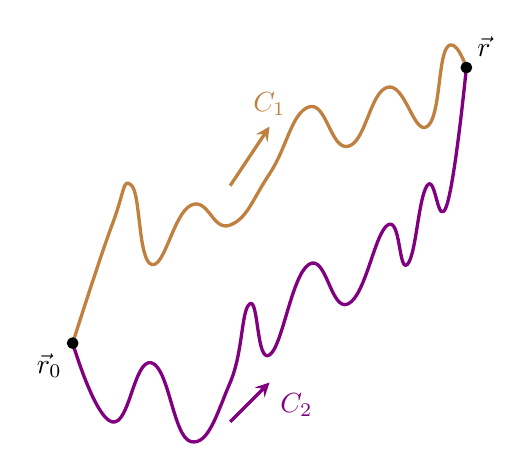
\begin{tikzpicture}[line width = 1.2pt, line join=round,x=0.5cm,y=0.5cm,>=stealth]
		% Koordinaten der Punkte
		\coordinate (a) at (0,0);
		\coordinate (b) at (10,7);
		% Weg 1
		\draw [color=brown] plot[smooth,tension=0.8] coordinates{(a) (1,3) (1.5,4) (2,2) (3,3.5) (4,3) (5,4.3) (6,6) (7,5) (8,6.5) (9,5.5) (9.5,7.5) (b)};
		\draw[->,color=brown] (4,4) -- (5,5.5) node[anchor=south] {$C_1$};
		% Weg 2
		\draw [color=violet] plot[smooth, tension=0.8] coordinates{(a) (1,-2) (2,-0.5) (3,-2.5) (4,-1) (4.5,1) (5,-0.3) (6,2) (7,1) (8,3) (8.5,2) (9,4) (9.5,3.5) (b)};
		\draw[->,color=violet] (4,-2) -- (5,-1) node[anchor=north west] {$C_2$};
		% Punkt 0
		\filldraw (a) circle (1.5pt);
		\draw (a) node[anchor=north east] {$\vec{r} _0$};
		% allgemeiner Punkt
		\filldraw (b) circle (1.5pt);
		\draw (b) node [anchor = south west] {$\vec{r} $};
	\end{tikzpicture}
	\hfill
	\begin{tikzpicture}[line width = 1.2pt,
			line join=round,
			scale=1,
			x=0.5cm,
			y=0.5cm,
			>=stealth]
		% Koordinaten der Punkte des Weges
		\coordinate (a) at (0,2);
		\coordinate (b) at (8,5);
		\coordinate (c) at (2,3);
		\coordinate (d) at (-2,4.3);
		\coordinate (e) at (9.6,2.5);

		% Rechte Winkel
		\draw (0.6,2.4) arc (10:120:0.4cm);
		\filldraw (0.05,2.6) circle (1pt);
		\draw (7.7,5.8) arc (120:210:0.4cm);
		\filldraw (7.62,5.2) circle (1pt);
		% Fläche 1
		\draw plot[smooth, tension = 0.8] coordinates{(-3,5) (a) (0,-2)};
		\draw [decorate, decoration={markings,
					mark=between positions 0.2 and 0.5 step 3mm with
						{\arrow[green]{latex}}}] plot[smooth, tension = 0.8] coordinates{(-3,5) (a) (0,-2)};
		\draw (0,-2) node[anchor=north] {$\phi(\vec{r} _0)$};
		% Fläche 2 
		\draw  plot[smooth, tension = 0.8] coordinates{(7,8) (b) (e) (10,2)};
		\draw  [decorate, decoration={markings,
					mark=between positions 0.6 and 0.95 step 3mm with
						{\arrow[green]{latex}}}] plot[smooth, tension = 0.8] coordinates{(7,8) (b) (e) (10,2)};
		\draw (10,2) node[anchor=north west] {$\phi(\vec{r} )$};
		% Punkte
		\draw (a) circle (1.5pt);
		\draw (a) node[anchor=north east] {$\vec{r} _1$};
		\draw (b) circle (1.5pt);
		\draw (b) node[anchor=south west] {$\vec{r} _2$};
		\draw (d) circle (1.5pt);
		\draw (d) node[anchor=south west] {$\vec{r} _0$};
		%\draw [color=green] plot[smooth] coordinates{(d) (f) (a)}; 

		\draw (e) node[anchor=north east] {$\vec{r} $};
		\draw (e) circle (1.5pt);

		% Weg
		\draw [color=magenta] plot[smooth, tension=0.8] coordinates{(a) (c) (6,4) (b)};
		\draw [decorate, , decoration={markings,
					mark=between positions 0.1 and 0.99 step 3mm with
						{\arrow[green]{latex}}}] plot[smooth, tension=0.8] coordinates{(a) (c) (6,4) (b)};
		\draw [->,color=magenta] (c) -- ++(3,{2/5*3}) node[anchor=south] {$\vec{E}$};
		\draw [->,color=blue] (c) -- ++(2,{2/5*2}) node[anchor=south east] {$\dd \vec{s}$};
	\end{tikzpicture}
\end{center}